\documentclass{article}
\usepackage{graphicx}
\usepackage{hyperref}
\usepackage{algorithm}
\usepackage{amsmath}
\usepackage{algpseudocode}
\usepackage[
    top=0.5in,
    bottom=0.9in,
    left=0.75in,
    right=0.75in
]{geometry}
\usepackage{color, colortbl}
\definecolor{LightYellow}{rgb}{1, 0.9, 0.78}

\title{\textbf{GPU Computing} \\
    \large Homework 1: Matrix Transposition \\
}
\author{Murtas Cristian \\ 248025 \\ cristian.murtas@studenti.unitn.it \\
\href{https://github.com/SecondarySkyler/gpu-computing/tree/main/matrix_transposition}{GitHub Repository}
} 

\begin{document}
\maketitle

\section{Problem Description}
The goal of this homework is to implement a matrix transposition algorithm, where the transpose of a matrix
is an operator which flips the matrix over its diagonal. That is, if $A$ is a matrix of size $m \times n$, then
the transpose of $A$ is a matrix of size $n \times m$ where the element at row $i$ and column $j$ of $A$, is the element at 
row $j$ and column $i$ of the transpose of $A$, also denoted as $A\textsuperscript{T}$. \\
Additionally, we are asked to measure the effective bandwidth of our implementation, considering also the
usage of different optimization flags such as: \texttt{-O0}, \texttt{-O1}, \texttt{-O2}, \texttt{-O3}. \\
Furthermore an analysis of the cache behavior of the algorithm is required, for this purpose we are going to use
valgrind.
\subsection{Algorithms}
In order to dimostrare qualcosa, two algorithms have been implemented: the first one is a na\"{i}ve approach, which
consists in iterating over the matrix and swapping the elements, while the second one is a more optimized version
which takes advantage of a block mechanism to reduce the number of cache misses.
\begin{algorithm}
    \caption{Na\"{i}ve Matrix Transposition}
    \begin{algorithmic}[1]
        \State $src \gets create\_matrix(size)$
        \For{$i = 0$ to $size$}
            \For{$j = 0$ to $size$}
                \State $dest[j * size + i] = src[i * size + j]$
            \EndFor
        \EndFor
    \end{algorithmic}
\end{algorithm}

\begin{algorithm}
    \caption{Matrix Transposition with Blocking}
    \begin{algorithmic}[1]
        \State $src \gets create\_matrix(size)$
        \For{$i = 0$ to $size$ increase $i$ by $block\_size$}
            \For{$j = 0$ to $size$ increase $j$ by $block\_size$}
                \For{$k = i$ to $i$ + $block\_size$} \Comment{Loop over the current block}
                    \For{$l = j$ to $j$ + $block\_size$}
                        \State $dest[l * size + k] = src[k * size + l]$
                    \EndFor
                \EndFor
            \EndFor
        \EndFor
    \end{algorithmic}
\end{algorithm}

\section{Experimental Setup}
\subsection{Hardware}
\begin{enumerate}
    \item \textbf{Desktop PC}
    \begin{itemize}
        \item \textbf{CPU}: AMD Ryzen 5 5600X
        \begin{itemize}
            \item \textbf{Cores}: 6
            \item \textbf{Threads}: 12
            \item \textbf{Base Clock}: 3.7 GHz
            \item \textbf{L1 Cache}: 64 KB (per core)
            \item \textbf{L2 Cache}: 512 KB (per core)
            \item \textbf{L3 Cache}: 32 MB
        \end{itemize}
        \item \textbf{RAM}: 16 GB DDR4
        \item \textbf{OS}: Ubuntu 22.04 (on WSL2)
    \end{itemize}
    \item \textbf{Marzola Cluster}
    \begin{itemize}
        \item \textbf{CPU}: Intel Xeon Silver 4309y
        \begin{itemize}
            \item \textbf{Cores}: 4
            \item \textbf{Threads}: 8
            \item \textbf{Base Clock}: 2.80 GHz
            \item \textbf{L1 Cache}: 32 KB (per core)
            \item \textbf{L2 Cache}: 1 MB (per core)
            \item \textbf{L3 Cache}: 12 MB
        \end{itemize}
    \end{itemize}
\end{enumerate}
\subsection{Results}
To provide a broader and precise analysis, the results have been collected executing both algorithms on matrices of different sizes,
ranging from $4 \times 4$ to $4096 \times 4096$. Also, for each dimension, the algorithms have been executed multiple times (100) to further improve the measurements. \\
The effective bandwidth has been calculated using the formula: \\
\begin{equation*}
    Effective \: Bandwidth = \frac{\left ( 2 * dimension * dimension * 4 \right )}{execution\: time}
    \left[\frac{GB}{s}\right]
\end{equation*}
where the factor $2$ is due to the fact that we are reading and writing the matrix, the $dimension$ is the size of the matrix, 
$4$ is the size of a single element (float) and the $execution \: time$ is the average of the 100 executions. \\
\subsubsection{Na\"{i}ve Algorithm}
The obtained results are in line with the expectations, indeed the executions with \texttt{-O0} don't show any significant difference because the compiler 
doesn't apply any optimization. Meanwhile, the executions with \texttt{-O1}, \texttt{-O2} and \texttt{-O3} show a significant improvement in the performance, on all
the tested platforms. This is probably due to the fact that the compiler is able to apply some optimizations, such as loop unrolling. \\
Another interesting aspect is that both the Ryzen 5 and the Xeon starts to show a decrease in the performance when the matrix size is greater than $64 \times 64$, 
as shown in figure \ref{fig:naive_comparison}. \\
To try to understand this behavior, the cache miss rate has been analyzed using valgrind (table \ref{tab:naive_cache_miss}). \\ 
\begin{table}[]
    \centering
    \begin{tabular}{|c|c|c|}
    \hline
    \multicolumn{3}{|c|}{\textbf{Ryzen 5 5600X}} \\
    \hline
    Dimension            & I1 miss rate & D1 miss rate \\ \hline
    64                   & 0.01\%       & 0.4\%        \\ \hline
    128                  & 0.00\%       & 4.0\%        \\ \hline 
    \end{tabular}
    \hspace{2em}
    \begin{tabular}{|c|c|c|}
        \hline
        \multicolumn{3}{|c|}{\textbf{Xeon 4309y}} \\
        \hline
        Dimension            & I1 miss rate & D1 miss rate \\ \hline
        64                   & 0.01\%       & 0.1\%        \\ \hline
        128                  & 0.00\%       & 3.6\%        \\ \hline 
    \end{tabular}
    \caption{Cache miss rate of the na\"{i}ve algorithm}
    \label{tab:naive_cache_miss}
\end{table}
\begin{figure}[H]
    \centering
    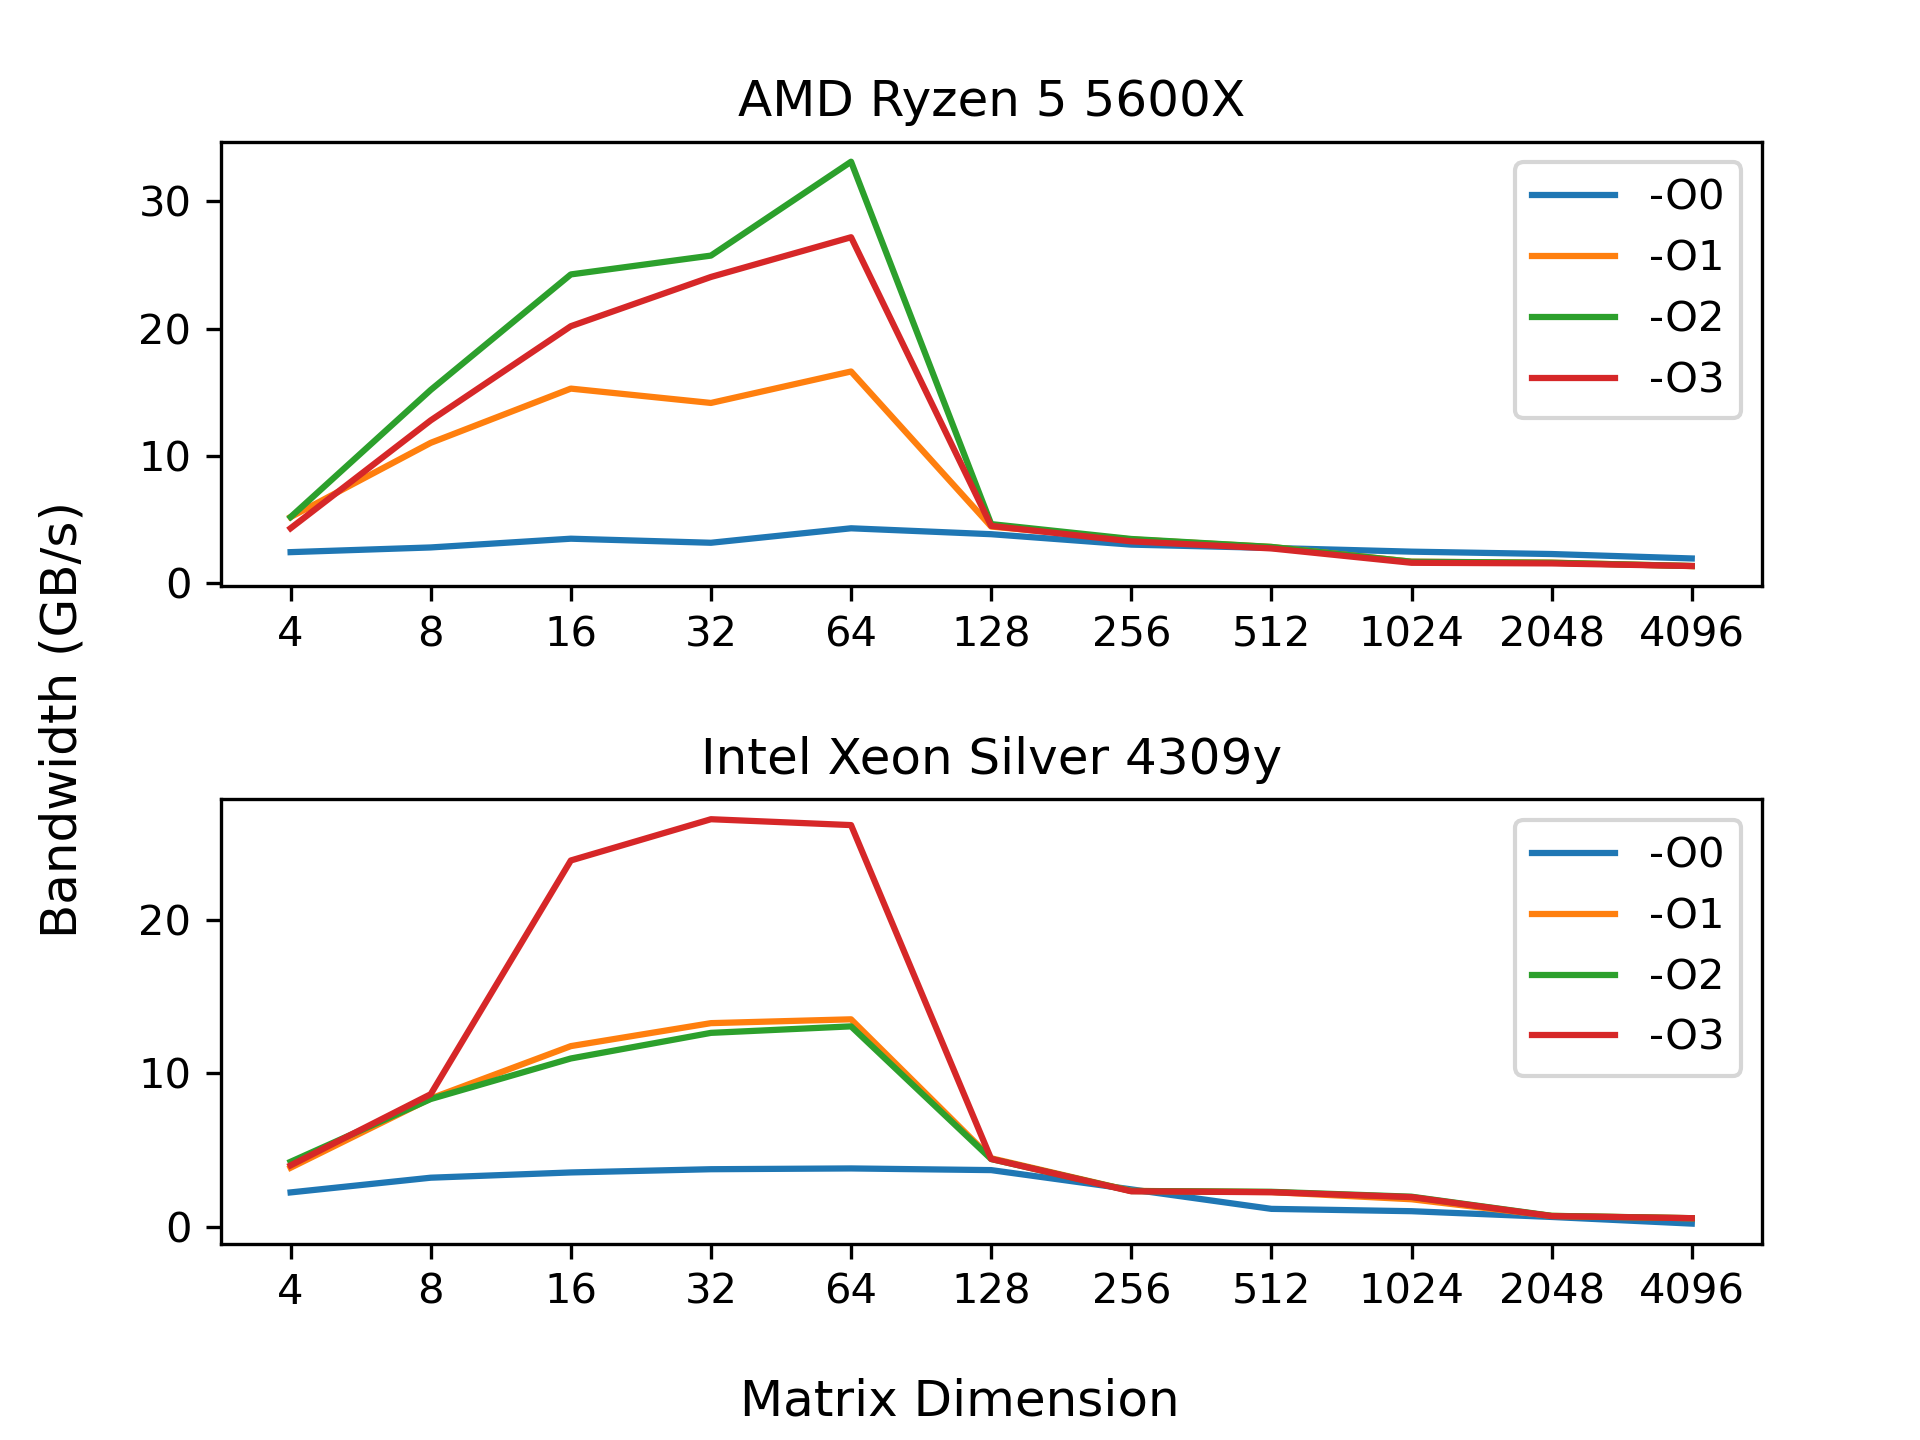
\includegraphics[scale=0.8]{report/img/naive_comparison.png}
    \caption{Comparison of the na\"{i}ve matrix transposition algorithm}
    \label{fig:naive_comparison}
\end{figure}
\subsubsection{Blocked Algorithm}
The idea behind the blocked algorithm is to reduce the number of cache misses by exploiting the locality of the data. But in order to benefit from this, the block
size must be chosen with care, furthermore the block size depends also on the size of the cache line. To decide the best size, the algorithm has been firstly
tested with different block sizes. The results for the different platforms are shown in table \ref{tab:blocked_results}, where the highlighted rows indicate the 
block size which fits the best for the given processor.
\begin{table}
    \centering
    \begin{tabular}{|c|c|}
        \hline
        \multicolumn{2}{|c|}{\textbf{Ryzen 5 5600X}} \\
        \hline
        Blocksize & Bandwidth \\ \hline
        2         & 4.8506 GB/s \\ \hline
        \rowcolor{LightYellow}
        4         & 7.49072 GB/s \\ \hline
        8         & 3.47782 GB/s \\ \hline
        16        & 3.62071 GB/s \\ \hline
        32        & 3.33045 GB/s \\ \hline
        64        & 2.7568 GB/s \\ \hline
    \end{tabular}
    \hspace{2em}
    \begin{tabular}{|c|c|}
        \hline
        \multicolumn{2}{|c|}{\textbf{Xeon 4309y}} \\
        \hline
        Blocksize & Bandwidth \\ \hline
        2         & 2.04391 GB/s \\ \hline
        4         & 3.83168 GB/s \\ \hline
        \rowcolor{LightYellow}
        8         & 4.80583 GB/s \\ \hline
        16        & 2.45955 GB/s \\ \hline
        32        & 2.59337 GB/s \\ \hline
        64        & 2.72063 GB/s \\ \hline
    \end{tabular}
    \caption{Results of the blocked algorithm with different block sizes ($1024 \times 1024$, \texttt{-O3})}
    \label{tab:blocked_results}
\end{table}
\begin{figure}[H]
    \centering
    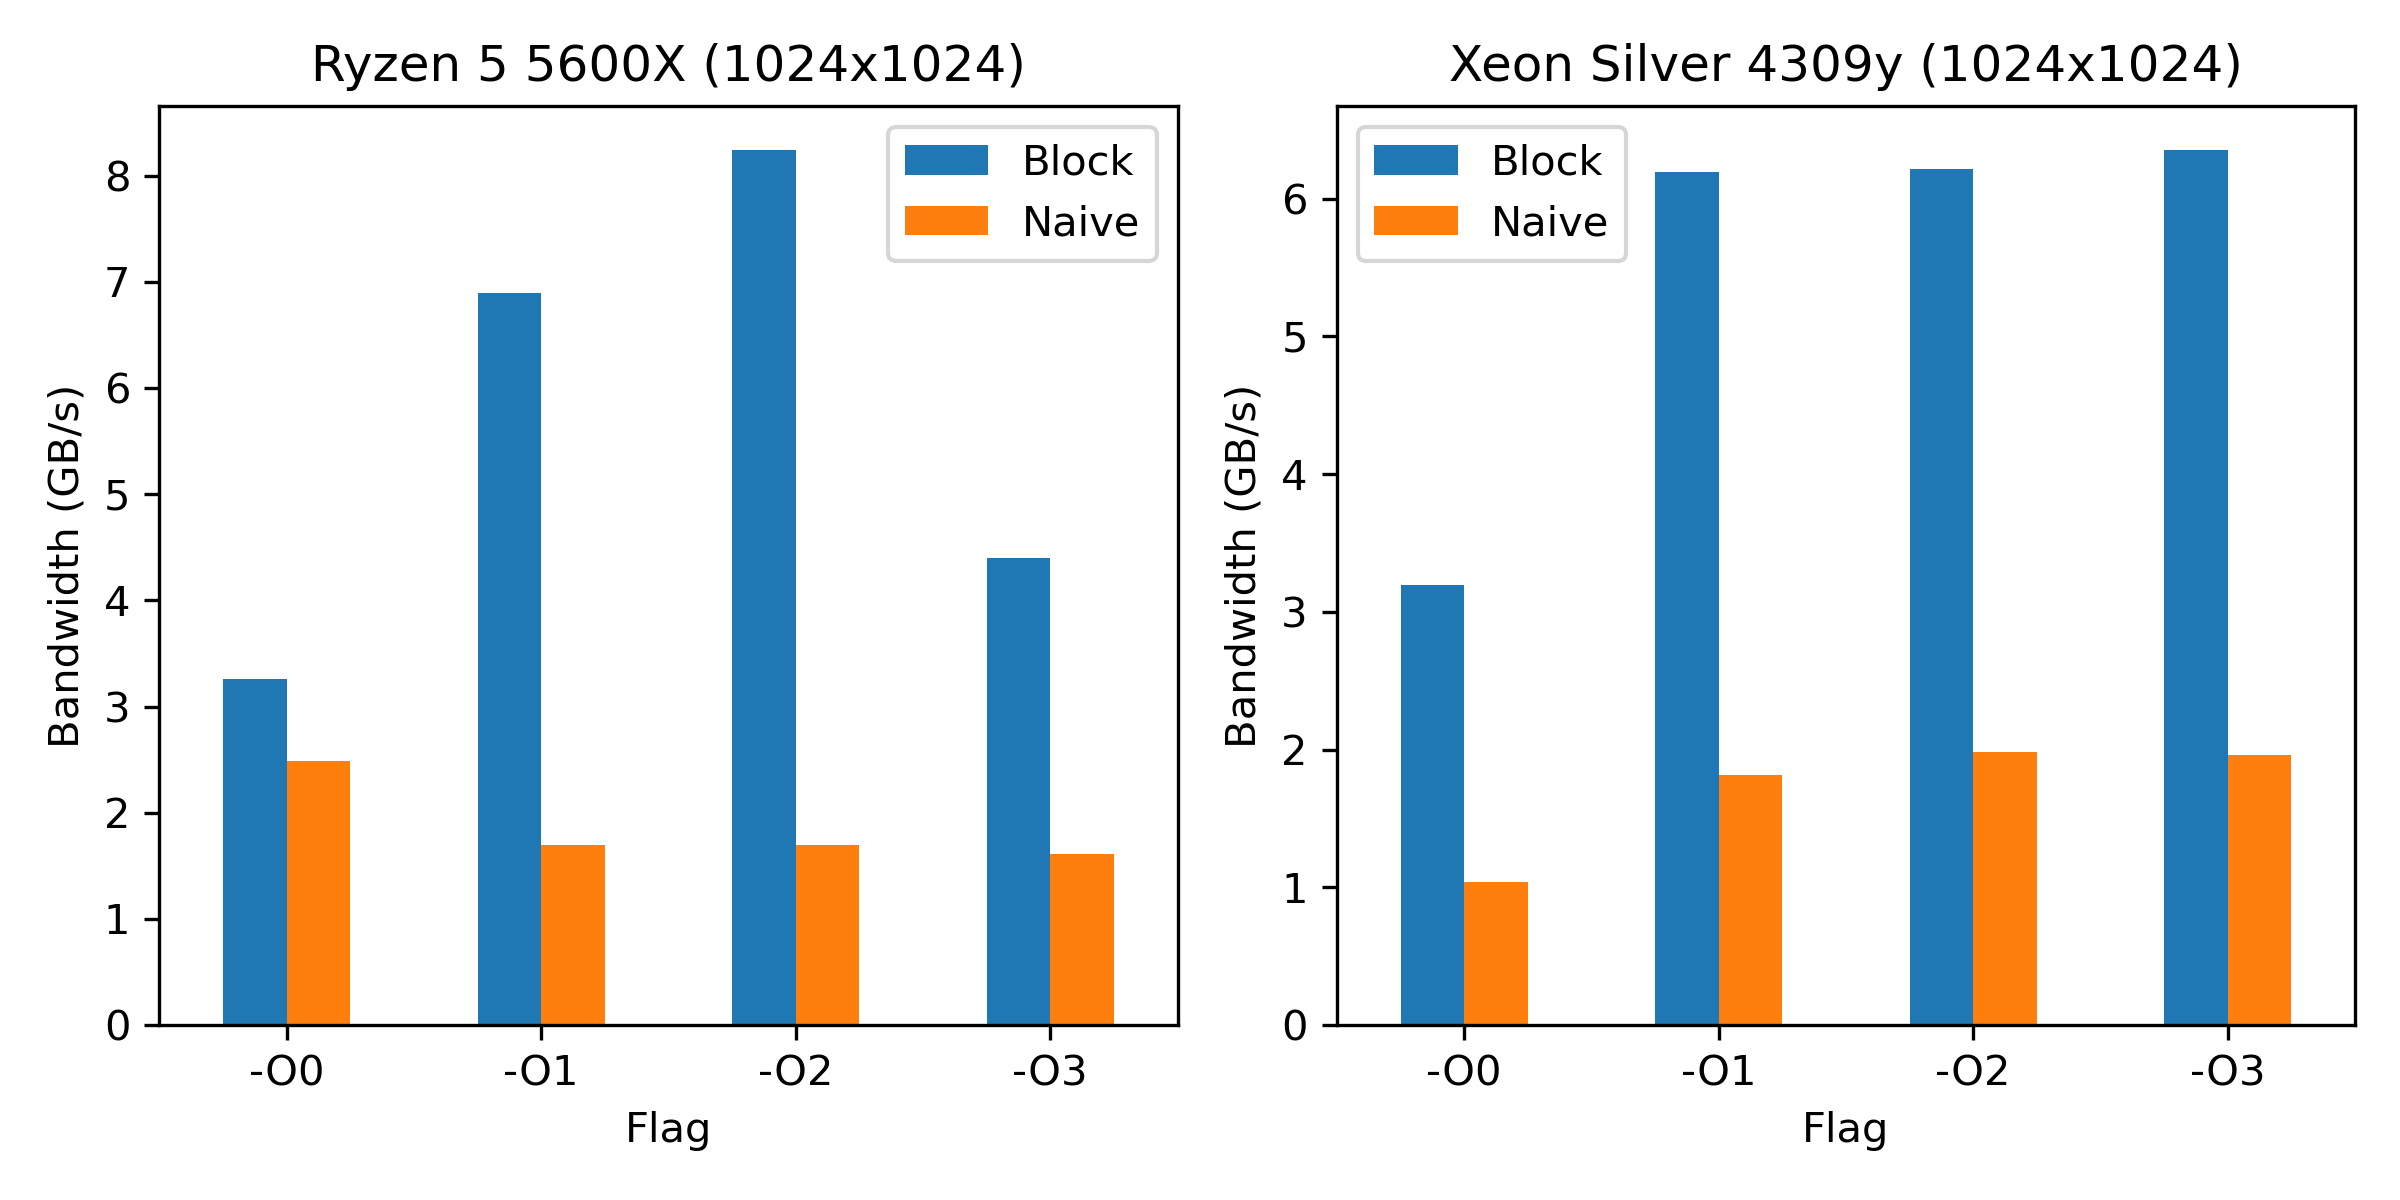
\includegraphics[width=0.85\textwidth]{report/img/block_vs_naive.png}
    \caption{Comparison of the blocked algorithm against the na\"{i}ve algorithm}
    \label{fig:blocked_comparison}
\end{figure}
\section{Conclusion}
\end{document}

